\documentclass{article}

\usepackage[LGR, T1]{fontenc} %για γλώσσα
\usepackage[greek,english]{babel}
\usepackage[utf8]{inputenc}

\usepackage{graphicx} % figures
\usepackage{caption}
\usepackage{subcaption}
\usepackage{float}
\usepackage{color}   %May be necessary if you want to color links
\usepackage{textcomp}
\usepackage{xcolor}

\usepackage{hyperref}
\usepackage{tocloft}
\usepackage{fontawesome5}

% Add dots to table of contents
\renewcommand{\cftsecleader}{\cftdotfill{\cftdotsep}}

\hypersetup{
    colorlinks=true,
    linkcolor=black,
    urlcolor=blue,
    citecolor=blue,
}

\begin{document}
\selectlanguage{Greek}
\begin{titlepage}

    \begin{figure}
        \centering
        
\includegraphics[scale=0.4]{Upatras}
    \end{figure}

    \begin{center}
        \line(1,0){300}\\
        [0.25in]
        \huge{\bfseries \selectlanguage{greek}Συλλογή δεδομένων για διπλωματική εργασία}\\

        \line(1,0){200}\\
        \begin{figure}[H]
            \centering
            
\includegraphics[scale=2.2]{logo}\\
        \end{figure}
    \end{center}

    \begin{flushright}
        \textsc{\\}
        \textsc{\\}

        \textsc{\large \\ Τριανταφυλλόπουλος Παναγιώτης\\ΑΜ 1054367}
        \textsc{\large \\ Τμήμα Μηχ. Η/Υ \& Πληροφορικής}
        \textsc{\large \\ Διπλωματική Εργασία}
    \end{flushright}

\end{titlepage}

\tableofcontents
\thispagestyle{empty}
\cleardoublepage

\setcounter{page}{1}
\selectlanguage{english}
\section*{Disclaimer}
\addcontentsline{toc}{section}{Disclaimer}

\selectlanguage{greek} Αυτό το ερευνητικό έργο θα χρησιμοποιήσει έναν τυχαία δημιουργημένο κωδικό αναγνώρισης για να διασφαλίσει την ανωνυμία όλων των συμμετεχόντων. Δε θα συλλεχθούν ούτε θα αποθηκευθούν προσωπικά στοιχεία ταυτοποίησης και δεν θα γίνει προσπάθεια σύνδεσης οποιουδήποτε συγκεκριμένου συμμετέχοντος με τις απαντήσεις ή τα δεδομένα του. Όλα τα δεδομένα που συλλέγονται κατά τη διάρκεια αυτής της μελέτης θα διατηρηθούν αυστηρά απόρρητα και θα χρησιμοποιηθούν αποκλειστικά για ερευνητικούς σκοπούς. Η συμμετοχή σε αυτή τη μελέτη είναι εντελώς εθελοντική και οι συμμετέχοντες μπορούν να αποσυρθούν ανά πάσα στιγμή χωρίς κυρώσεις ή απώλεια ωφελημάτων που διαφορετικά δικαιούνται.

\section*{Εισαγωγή}
\addcontentsline{toc}{section}{Εισαγωγή}

Καλείστε να συμμετάσχετε στη συλλογή δεδομένων στα πλαίσια της διπλωματικής εργασίας του προπτυχιακού φοιτητή Τριανταφυλλόπουλου Παναγιώτη, η οποία έχει σκοπό τη δημιουργία ενός συστήματος συστάσεων ιστοσελίδων. Για τη συλλογή δεδομένων θα χρειαστείτε έναν φυλλομετρητή (\selectlanguage{english}Google Chrome\selectlanguage{greek} ή \selectlanguage{english}Firefox\selectlanguage{greek}) και να εγκαταστήσετε και να χρησιμοποιήσετε μία επέκταση φυλλομετρητή (\selectlanguage{english}browser extension\selectlanguage{greek}) που έχει δημιουργηθεί από τον φοιτητή. Για να συγκεντωρθεί επαρκές μέγεθος δεδομένων θα χρειαστεί να χρησιμοποιείτε την επέκταση για μία εβδομάδα (7 ημέρες) κατά την περιήγησή σας στο διαδίκτυο.

\section*{Σκοπός συλλογής δεδομένων}
\addcontentsline{toc}{section}{Σκοπός συλλογής δεδομένων}

Ο σκοπός της συλλογής δεδομένων από χρήστες που χρησιμοποιούν την επέκταση φυλλομετρητή είναι η ανάπτυξη ενός συστήματος συστάσεων. Αυτό το σύστημα θα μπορεί να προτείνει ποιοι υπερσύνδεσμοι (\selectlanguage{english}URLs\selectlanguage{greek}) ενός ιστοτόπου είναι πιο πιθανό να ενδιαφέρουν το χρήστη. Τα δεδομένα που συλλέγονται θα αναλυθούν χρησιμοποιώντας αλγόριθμους μηχανικής μάθησης για τον εντοπισμό μοτίβων και τάσεων στη συμπεριφορά των χρηστών. Στη συνέχεια, αυτές οι πληροφορίες θα χρησιμοποιηθούν για την εκπαίδευση του συστήματος συστάσεων ώστε να κάνει πιο ακριβείς και χρήσιμες προτάσεις.
\section*{Οδηγίες Εγκατάστασης}
\addcontentsline{toc}{section}{Οδηγίες Εγκατάστασης}

Αρχικά θα χρειαστείτε ένα φυλλομετρητή (\selectlanguage{english}Google Chrome\selectlanguage{greek} ή \selectlanguage{english}Firefox\selectlanguage{greek}). Αν δεν έχετε ήδη κάποιον από τους δύο φυλλομετρητές μπορείτε να εγκαταστήσετε το φυλλομετρητή \selectlanguage{english}Google Chrome\selectlanguage{greek} πατώντας \href{https://www.google.com/chrome/}{εδώ} και τον \selectlanguage{english}Firefox\selectlanguage{greek} πατώντας \href{https://www.mozilla.org/el/firefox/new/}{εδώ}. Για να κατεβάσετε το αρχείο εγκατάστασης του φυλλομετρητή αρκεί να πατήσετε το κουμπί στο οποοίο δείχνει το βέλος στις παρακάτω εικόνες. Μόλις κατεβάσετε το αρχείο αρκεί να το εκτελέσετε και να ακολουθήσετε τις οδηγίες μέχρι να φτάσετε στο τέλος.

\begin{figure}[H]
    \centering
    \begin{subfigure}{.45\textwidth}
        \includegraphics[width=\textwidth]{googlechromeinstallation}
        \caption{\selectlanguage{english}Google Chrome\selectlanguage{greek}}
        \label{Fig:sub1}
    \end{subfigure}
    \hfill
    \begin{subfigure}{.45\textwidth}
        \includegraphics[width=\textwidth]{firefoxinstallation}
        \caption{\selectlanguage{english}Firefox\selectlanguage{greek}}
        \label{Fig:sub2}
    \end{subfigure}
\end{figure}

% todo add explanation how to download the extension
\selectlanguage{english}
\subsection*{Google Chrome}
\addcontentsline{toc}{subsection}{Google Chrome}

\selectlanguage{greek}Για να κατεβάσετε την επέκταση που λειτουργεί για το φυλλομετρητή \selectlanguage{english}Google Chrome\selectlanguage{greek} αρκεί να πατήσετε \href{https://drive.google.com/drive/folders/1JhenJNu0teL6oo55IWzdhamBNJH3g-d_?usp=share_link}{εδώ} και να κατεβάσετε το φάκελο \selectlanguage{english}Url\_Rating\selectlanguage{greek}. Αυτό γίνεται πατώντας στις τρεις κουκίδες στα δεξιά από το όνομα του φακέλου και στη συνέχεια πατώντας λήψη όπως φαίνεται στην παρακάτω εικόνα.

\begin{figure}[H]
    \centering
    \includegraphics[width=\textwidth]{downloadchrome}
    \caption*{Λήψη επέκτασης για \selectlanguage{english}Google Chrome\selectlanguage{greek}}
\end{figure}

\selectlanguage{greek}Αν έχετε το φυλλομετρητή \selectlanguage{english}Google Chrome\selectlanguage{greek}, ανοίξτε το φυλλομετρητή σας και μεταβείτε στη σελίδα των επεκτάσεων. Αυτό μπορείτε να το κάνετε πληκτρολογώντας \selectlanguage{english}chrome://extensions\selectlanguage{greek} στη γραμμή διευθύνσεων ή κάνοντας κλικ στο μενού με τις τρις κουκκίδες στην πάνω δεξιά γωνία και επιλέγοντας \textbf{Περρισσότερα Εργαλεία $\rightarrow$ Επεκτάσεις} όπως φαίνεται στις παρακάτω εικόνες. 

\begin{figure}[H]
    \centering
    \begin{minipage}[t]{0.45\textwidth}
        \centering
        \begin{subfigure}[t]{\textwidth}
            \includegraphics[width=\textwidth]{addressbar}
            \caption{\selectlanguage{english}chrome://extensions\selectlanguage{greek} στη γραμμή διευθύνσεων}
            \label{Fig:addressbar}
        \end{subfigure}
        \vspace{\fill}
    \end{minipage}
    \hfill
    \begin{minipage}{0.45\textwidth}
        \begin{subfigure}{\textwidth}
            \includegraphics[width=\textwidth]{moretools}
            \caption{Περρισσότερα Εργαλεία $\rightarrow$ Επεκτάσεις}
            \label{Fig:moretools}
        \end{subfigure}
    \end{minipage}
\end{figure}

Θα πρέπει να έχετε μπροστά σας την παρακάτω οθόνη με τις δικές σας εγκατεστημένες επεκτάσεις.

\begin{figure}[H]
    \includegraphics[width=\textwidth]{chromeextensions}
    \caption*{Αρχική οθόνη \selectlanguage{english}chrome://extensions\selectlanguage{greek}}
\end{figure}

Στη συνέχεια πρέπει να ενεργοποιήσετε τη λειτουργία για προγραμματιστές. Ο τρόπος για να γίνει αυτό είναι κανοντας κλικ στον διακόπτη στην πάνω δεξιά γωνία της σελίδας όπως φαίνεται στις παρακάτω εικόνες.
\begin{figure}[H]
    \centering
    \begin{subfigure}{0.45\textwidth}
        \includegraphics[width=\textwidth]{devoff}
        \caption{Λειτουργία για προγραμματιστές ανενεργή}
        \label{Fig:devoff}
    \end{subfigure}
    \hfill
    \begin{subfigure}{0.45\textwidth}
        \includegraphics[width=\textwidth]{devon}
        \caption{Λειτουργία για προγραμματιστές ενεργή}
        \label{Fig:devon}
    \end{subfigure}
\end{figure}

Μετά πρέπει να φορτώσετε την επέκταση στον \selectlanguage{english}Google Chrome\selectlanguage{greek}. Για να γίνει αυτό πρέπει να πατήσετε στο κουμπί \textbf{Φόρτωση ανεπτυγμένης επέκτασης} (το οποίο εμφανίστηκε αφού ενεργοποιήσατε τη λειτουργία για προγραμματιστές) στο πάνω αριστερό μέρος της σελίδας και να επιλέξετε το φάκελο που έχετε την επέκταση.
\begin{figure}[H]
    \centering
    \begin{minipage}[t]{0.45\textwidth}
        \centering
        \begin{subfigure}[t]{\textwidth}
            \includegraphics[width=\textwidth]{loadunpacked}
        \caption{Φόρτωση ανεπτυγμένης επέκτασης}
        \label{Fig:loadunpacked}
        \end{subfigure}
        \vspace{\fill}
    \end{minipage}
    \hfill
    \begin{minipage}{0.45\textwidth}
        \begin{subfigure}{\textwidth}
            %todo: change it to the correct folder name
            \includegraphics[width=\textwidth]{choosefolder}
            \caption{Επιλογή φακέλου}
            \label{Fig:choosefolder}
        \end{subfigure}
    \end{minipage}
\end{figure}

Η επέκταση θα πρέπει να έχει εκγατασταθεί με επιτυχία και να βλέπετε την παρακάτω οθόνη
\begin{figure}[H]
    \includegraphics[width=\textwidth]{installedextensionchrome}
    \caption*{Επέκταση εγκατεστημένη}
\end{figure}

\cleardoublepage
\selectlanguage{english}
\subsection*{Firefox}
\addcontentsline{toc}{subsection}{Firefox}
\selectlanguage{greek}

Για να κατεβάσετε την επέκταση που λειτουργεί για το φυλλομετρητή \selectlanguage{english}Firefox\selectlanguage{greek} αρκεί να πατήσετε \href{https://drive.google.com/drive/folders/191-K02IJk3PNCtMcF94pB9eTDhVBnS2K?usp=share_link}{εδώ} και να κατεβάσετε το αρχείο \selectlanguage{english}url\_rating.xpi\selectlanguage{greek}. Αυτό γίνεται πατώντας στις τρεις κουκίδες στα δεξιά από το όνομα του αρχείου και στη συνέχεια πατώντας λήψη όπως φαίνεται στην παρακάτω εικόνα.

\begin{figure}[H]
    \centering
    \includegraphics[width=\textwidth]{downloadfirefox}
    \caption*{Λήψη επέκτασης για \selectlanguage{english}Firefox\selectlanguage{greek}}
\end{figure}

\selectlanguage{greek}Για να εγκαταστήσετε την επέκταση στον \selectlanguage{english}Firefox\selectlanguage{greek}, ανοίξτε το φυλλομετρητή σας και μεταβείτε στη σελίδα των επεκτάσεων. Αυτό μπορείτε να το κάνετε πληκτρολογώντας \selectlanguage{english}about://addons\selectlanguage{greek} στη γραμμή διευθύνσεων ή κάνοντας κλικ στο μενού με τις τρις οριζόντιες γραμμές στην πάνω δεξιά γωνία και επιλέγοντας \textbf{Πρόσθετα και Θέματα} όπως φαίνεται στις παρακάτω εικόνες. 

\begin{figure}[H]
    \centering
    \begin{minipage}[t]{0.45\textwidth}
        \centering
        \begin{subfigure}[t]{\textwidth}
            \includegraphics[width=\textwidth]{aboutaddons}
        \caption{\selectlanguage{english}about://addons\selectlanguage{greek} στη γραμμή διευθύνσεων}
        \label{Fig:aboutaddons}
        \end{subfigure}
        \vspace{\fill}
    \end{minipage}
    \hfill
    \begin{minipage}{0.45\textwidth}
        \begin{subfigure}{\textwidth}
            \includegraphics[width=\textwidth]{addonsthemes}
            \caption{Πρόσθετα και Θέματα}
            \label{Fig:addonsthemes}
        \end{subfigure}
    \end{minipage}
\end{figure}

Θα πρέπει να έχετε μπροστά σας την παρακάτω οθόνη.

\begin{figure}[H]
    \includegraphics[width=\textwidth]{firefoxextensions}
    \caption*{Διαχείριση Επεκτάσεων}
\end{figure}

Πατήστε στο γρανάζι (\faCog) όπως φάινεται στην παρακάτω εικόνα και επιλέξτε \textbf{εγκατάσταση πρόσθετου από αρχείο}. Επιλέγετε το αρχείο που κατεβάσατε νωρίτερα με κατάληξη \selectlanguage{english}.xpi\selectlanguage{greek}.

\begin{figure}[H]
    \centering
    \begin{minipage}[t]{0.45\textwidth}
        \centering
        \begin{subfigure}[t]{\textwidth}
            \includegraphics[width=\textwidth]{installfromfile}
        \caption{Eγκατάσταση πρόσθετου από αρχείο}
        \label{Fig:installfromfile}
        \end{subfigure}
        \vspace{\fill}
    \end{minipage}
    \hfill
    \begin{minipage}{0.45\textwidth}
        \begin{subfigure}{\textwidth}
            %todo: change it to the correct file name
            \includegraphics[width=\textwidth]{choosefolder}
            \caption{Επιλογή αρχείου}
            \label{Fig:choosefile}
        \end{subfigure}
    \end{minipage}
\end{figure}

Ο \selectlanguage{english}Firefox\selectlanguage{greek} θα εμφανίσει ένα προειδοποιητικό μήνυμα το οποίο σας ζητά να επιβεβαιώσετε την εγκατάσταση. Κάντε κλικ στο \textquotedblleftΠροσθήκη\textquotedblright για να προχωρήσετε. Η επέκταση θα έχει πλέον εγκατασταθεί και θα πρέπει να βλέπετε τα παρακάτω.

\begin{figure}[H]
    \includegraphics[width=\textwidth]{installedextensionfirefox}
    \caption*{Πρόσθετο εγκατεστημένο}
\end{figure}

\section*{Οδηγίες Χρήσης}
\addcontentsline{toc}{section}{Οδηγίες Χρήσης}

Αρχικά μπορείτε ανά πάσα στιγμή να βεβαιωθείτε ότι έχετε εγκαταστήσει την επέκταση πατώντας το εικονίδιο με το κομμάτι παζλ στο πάνω δεξί μέρος της οθόνης. Θα πρέπει να φαίνεται η επέκταση \selectlanguage{english}Url Rating\selectlanguage{greek} (με εικονίδιο ένα αστέρι) μαζί με τις υπόλοιπες επεκτάσεις που έχετε ήδη εγκαταστήσει (αν έχετε), όπως φαίνεται παρακάτω.

\begin{figure}[H]
    \centering
    \begin{minipage}[t]{0.45\textwidth}
        \centering
        \begin{subfigure}[t]{\textwidth}
            \includegraphics[width=\textwidth]{chromeextension}
        \caption{Επεκτάσεις στον \selectlanguage{english}Google Chrome\selectlanguage{greek}}
        \label{Fig:chromeextension}
        \end{subfigure}
        \vspace{\fill}
    \end{minipage}
    \hfill
    \begin{minipage}[t]{0.45\textwidth}
        \centering
        \begin{subfigure}[t]{\textwidth}
            \includegraphics[width=\textwidth]{firefoxextension}
            \caption{Επεκτάσεις στον \selectlanguage{english}Firefox\selectlanguage{greek}}
            \label{Fig:firefoxextension}
        \end{subfigure}
    \end{minipage}
\end{figure}

Πατώντας πάνω στην επέκταση θα σας εμφανιστεί η αρχική της οθόνη:

\begin{figure}[H]
    \centering
    \begin{minipage}[t]{0.45\textwidth}
        \centering
        \begin{subfigure}[t]{\textwidth}
            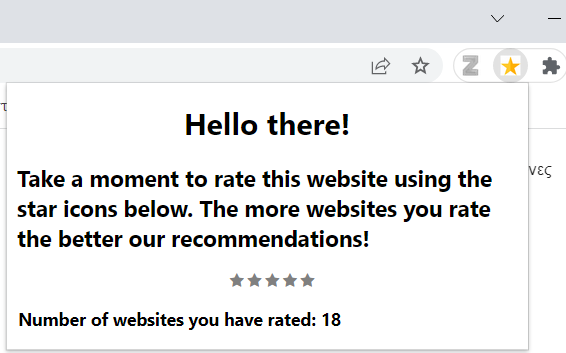
\includegraphics[width=\textwidth]{chromestartpage}
        \caption{Αρχική οθόνη \selectlanguage{english}Google Chrome\selectlanguage{greek}}
        \label{Fig:chromestartpage}
        \end{subfigure}
        \vspace{\fill}
    \end{minipage}
    \hfill
    \begin{minipage}[t]{0.45\textwidth}
        \centering
        \begin{subfigure}[t]{\textwidth}
            \includegraphics[width=\textwidth]{firefoxstartpage}
            \caption{Αρχική οθόνη \selectlanguage{english}Firefox\selectlanguage{greek}}
            \label{Fig:firefoxstartpage}
        \end{subfigure}
    \end{minipage}
\end{figure}

Για να αξιολογήσετε μία ιστοσελίδα αρκεί να πατήσετε ένα από τα αστέρια που στο κάτω μέρος της αρχικής οθόνης. Για τη χειρότερη αξιολόγηση (βαθμολογία 1) πατάτε το αστέρι που βρίσκεται στα αριστερά ενώ για την καλύτερη αξιολόγηση (βαθμολογία 5) πατάτε το αστέρι που βρίσκεται στα δεξιά. Όταν αξιολογήσετε μία ιστοσελίδα θα σας εμφανιστεί μήνυμα επιτυχίας, όπως φαίνεται στις εικόνες παρακάτω.

\begin{figure}[H]
    \centering
    \begin{minipage}[t]{0.45\textwidth}
        \centering
        \begin{subfigure}[t]{\textwidth}
            \includegraphics[width=\textwidth]{chromesuccess}
        \caption{Επιτυχής εξιολόγηση \selectlanguage{english}Google Chrome\selectlanguage{greek}}
        \label{Fig:chromesuccess}
        \end{subfigure}
        \vspace{\fill}
    \end{minipage}
    \hfill
    \begin{minipage}[t]{0.45\textwidth}
        \centering
        \begin{subfigure}[t]{\textwidth}
            \includegraphics[width=\textwidth]{firefoxsuccess}
            \caption{Επιτυχής αξιολόγηση \selectlanguage{english}Firefox\selectlanguage{greek}}
            \label{Fig:firefoxsuccess}
        \end{subfigure}
    \end{minipage}
\end{figure}

Σε περίπτωση που προσπαθήσετε να αξιολογήσετε μία ιστοσελίδα που δεν είναι έγκυρη (π.χ. μία κενή ιστοσελίδα) θα εμφανιστεί μήνυμα αποτυχίας όπως φαίνεται παρακάτω.

\begin{figure}[H]
    \centering
    \begin{minipage}[t]{0.45\textwidth}
        \centering
        \begin{subfigure}[t]{\textwidth}
            \includegraphics[width=\textwidth]{chromefailure}
        \caption{Αποτυχημένη εξιολόγηση \selectlanguage{english}Google Chrome\selectlanguage{greek}}
        \label{Fig:chromefailure}
        \end{subfigure}
        \vspace{\fill}
    \end{minipage}
    \hfill
    \begin{minipage}[t]{0.45\textwidth}
        \centering
        \begin{subfigure}[t]{\textwidth}
            \includegraphics[width=\textwidth]{firefoxfailure}
            \caption{Αποτυχημένη αξιολόγηση \selectlanguage{english}Firefox\selectlanguage{greek}}
            \label{Fig:firefoxfailure}
        \end{subfigure}
    \end{minipage}
\end{figure}

\end{document}

